\documentclass{article}
\usepackage[utf8]{inputenc}

\usepackage{mathtools}
\usepackage{amsthm}
\usepackage{graphicx}
\usepackage{hyperref}
\usepackage{xcolor}

\usepackage[T1]{fontenc}

\title{FYS1210 Oblig 1/ Lab 1}
\author{Samuel Bigirimana}



\begin{document}
    \maketitle
    \textbf{Sammendrag}
    \begin{verbatim}
        Denne rapporten viser mitt arbeid med Lab 1, hvor jeg 
        etter beste evne har prøvd å finne og bruke matematiske 
        teorier for så å simulere dem også til slutt lage reelle 
        kretser. Her har jeg fokusert på å bli kjent med verktøy 
        som CercuitLab, Multimeter, motstandere, kretsbrett osv.
    \end{verbatim}

    \raggedright
    \section*{1. Introduksjon}
        Formålet med denne labøvelsen er å få noen grunnleggende 
        ferdigheter innen elektronikk. Jeg skal lære om sammenhengen mellom matematisk  
        analyse, simulering  og  reelle  kretser.
    
    \subsection*{1.2 Læringsmål}
        • Danne kobling mellom elektrisk skjema og elektriske kretser. \linebreak
        • Bli kjent med strømmåling, spenningsmåling og motstandsmåling. \linebreak
        • Kunne beregne, simulere og koble opp og måle på flere elektriske
        kretserfor og se at teori, simulering og praksis henger sammen. \linebreak
        • Kunne  forstå at utgangsmotstand og inngangsmotstand påvirker 
        signaloverført fra kilde til last. Her er kilde batteri og last 
        motstand.
    \pagebreak

    \section*{2. Teori}
        \textbf{Dette er formlene jeg brukte under LAB 1 øvelsen:} \linebreak
        Formel for V gitt I og R (viser også hvordan man kan bruke formelen for å finne I og R):
        \begin{equation}
            \begin{split}
                V &= R * I \\
                -> I &= \dfrac{V}{R} \\
                -> R &= \dfrac{V}{I}
            \end{split}
        \end{equation}

        Formel for utregning av motstand som er seriekoblet:
        \begin{equation}
            R_S = R_1 + R_2 + ... + R_n
        \end{equation}

        Formel for utregning av motstand som er parallellkoblet:
        \begin{equation}
            \dfrac{1}{R_P} = \dfrac{1}{R_1} + \dfrac{1}{R_2} + ... + \dfrac{1}{R_n}
        \end{equation}

    \section*{3. Metode}
        \subsection*{Oppg. 1:}
            \textbf{1a)} \linebreak
            › Siden at jeg skal måle en batteri som gir likespenning på 9v, vrir jeg velgeren 
            til "V="-området og tallet 20. \linebreak
            › Så kobler jeg sort måleledning til COM på multimeteret, og rød i hullet til høyre. \linebreak
            › Holder til slutt måleledningene borti batteriets poler, svart til "-" og rød til "+". \linebreak
            
            \textbf{1b)} \linebreak
            › Starter først med å velge meg 10 vilkårlige motstander \linebreak
            › Brukte Latex til å lage tabellen og  \href{https://en.wikipedia.org/wiki/Electronic_color_code}{denne siden} 
            for å tolke fargenene \linebreak
            › Vrir  multimeterets  funksjonsvelger  til  områadet  merket Ω og velger "motstandsverdi" etter det jeg tenker passer 
            best ift. fargekodene.
            \pagebreak

            \textbf{1c)} \linebreak
            Bruker formel (1): \linebreak
            \begin{equation}
                \begin{split}
                    I &= \dfrac{9V}{1k\Omega} \\
                    I &= 9mA
                \end{split}
            \end{equation} \linebreak

             Dette er det jeg simulerte inn i CircuitLab: \linebreak
            \begin{center}
                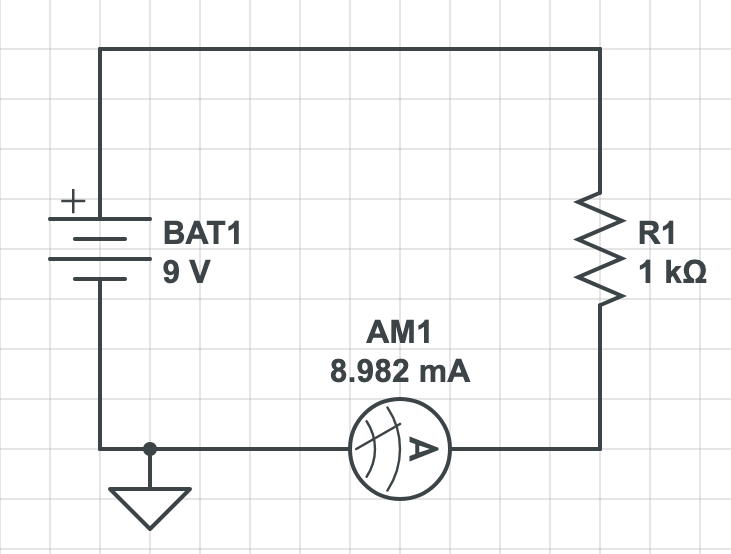
\includegraphics[scale=0.5]{vedlegg/1c.png}\linebreak
                \textit{\textcolor{gray}{Figur 1: Skjematisk oppsett av kretsen i oppgave 1c. Figuren er tegnet i CircuitLab.}}
            \end{center} 
            
            Koblet til slutt opp kretsen på koblingsbrettet og målte strømmen med multimeret.
        
        \subsection*{Oppg. 2:}
            Ved å bruke formel (2) for seriekoblede kretser, får jeg:
            \begin{equation*}
                \begin{split}
                    R_S &= 1k\Omega + 3.3k\Omega \\
                        &= 4.3k\Omega
                \end{split}
            \end{equation*}
            
            Regner deretter I med formel (1):
                \begin{equation*}
                    \begin{split}
                        I &= \dfrac{9V}{4.3k\Omega} \\
                            &\approx 2.1mA
                    \end{split}
                \end{equation*}
            
            Bruker til slutt strømmen som går gjennom R1 og R2 for å bestemme spenningsfallene med formel (1):
                \begin{equation*}
                    \begin{split}
                        V_{R1} &= 2.1mA * 1k\Omega \\
                            &\approx 2.1V \\
                            \\
                        V_{R2} &= 2.1mA * 3.3k\Omega \\
                            &\approx 6.9V
                    \end{split}
                \end{equation*}

            Simulasjonen i CircuitLab:
            \begin{center}
                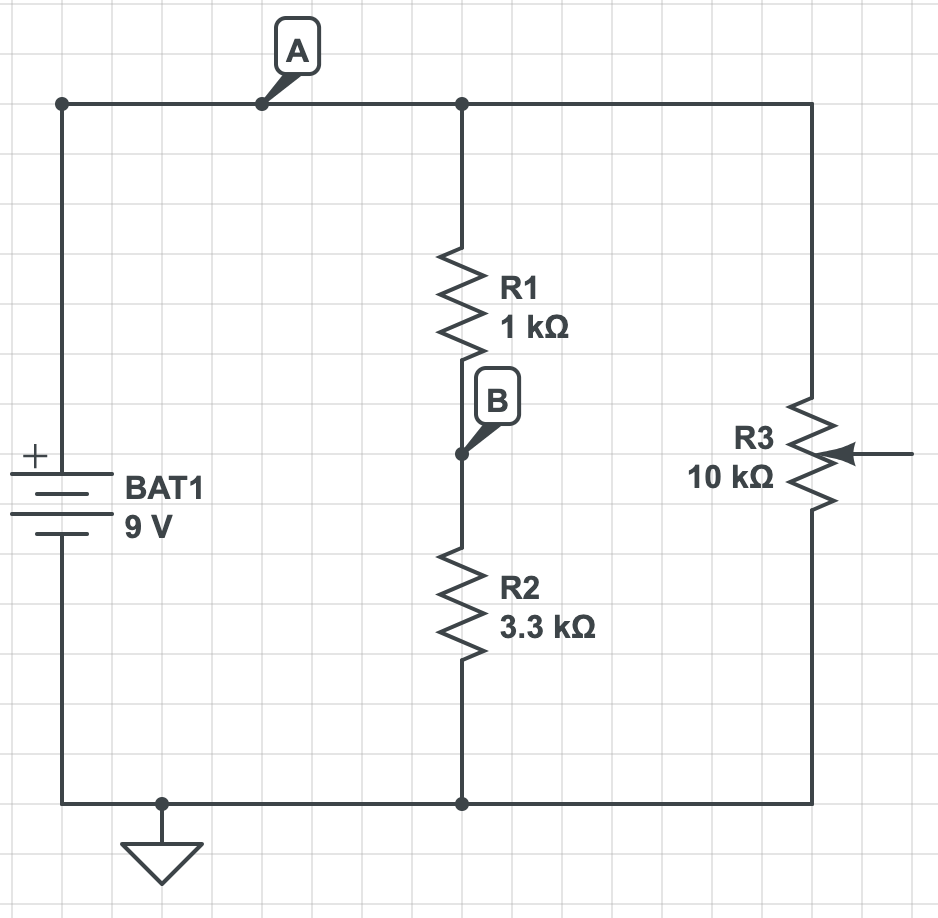
\includegraphics[scale=0.5]{vedlegg/2.png}\linebreak
                \textit{\textcolor{gray}{Figur 3: Skjematisk oppsett av kretsen i oppgave 2. Figuren er tegnet i CircuitLab.}}
            \end{center}
            
            \subsection*{Oppg. 3:}
                Starter først med å forenkle kretsen ved å finne total motstand. Her bruker jeg formlene (2) og (3): 
                \begin{equation*}
                    \begin{split}
                        R_{45} &= \dfrac{1}{(\dfrac{1}{3.3k\Omega})+(\dfrac{1}{3.3k\Omega})} \\
                            &\approx 1.65k\Omega \\
                            \\
                        R_{345} &= R_3 + R_{45} \\
                                &= 10k\Omega + 1.65k\Omega \\
                                &= 11.65k\Omega \\
                                \\
                        R_{2345} &= R_2 + R_{345} \\
                                &= \dfrac{1}{(\dfrac{1}{10k\Omega})+(\dfrac{1}{11.65k\Omega})} \\
                                &= 5.4k\Omega \\
                                \\
                        R_{tot} &= R_1 + R_{2345} \\
                            &= 1k\Omega + 5.4k\Omega \\
                            &= 6.4k\Omega
                    \end{split}
                \end{equation*}

                Finner deretter den totale strømmen gjennom kretsen ved å bruke formel (1):
                    \begin{equation*}
                        \begin{split}
                            I_{tot} &= \dfrac{V}{R_{tot}} \\
                                &= \dfrac{9V}{6.4k\Omega} \\
                                &\approx 6.4mA
                        \end{split}
                    \end{equation*}
                
                Nå som jeg har funnet hovedstrømmen kan jeg dekomponere den og finne strømmen i hver motstand:
                    \begin{equation*}
                        \begin{split}
                            -V_{R_1} &= I_{tot} * R_1 \\
                                    &= 1.4mA * 1k\Omega \\
                                    &= -1.4V \\
                                    \\
                            I_{R_1} &= I_{tot} \\
                                    &= 1.4mA
                        \end{split}
                    \end{equation*}

                Siden at den første motstanden gir et spenningsfall på 1.4V, 
                står vi igjen med spenningen \(V_{R1} = 7.6V\) \linebreak

                Regner dermed videre med gjenstående spenning på strømmen i \(R_2\) og \(R_{345}\):

                    \begin{equation*}
                        \begin{split}
                            I_{R_2} &= \dfrac{V_{R1}}{R_2} \\
                            &= \dfrac{7.6V}{10k\Omega} \\
                            &= 0.76mA \\
                            \\
                            I_{R_{345}} &= \dfrac{V_{R1}}{R_{345}} \\
                                    &= \dfrac{7.6V}{11.65k\Omega} \\
                                    &= 0.65mA
                        \end{split}
                    \end{equation*}
                
                    Utfra strømmen som går i \(R_3\) regner jeg ut spenningssfallet og \(V_{R_1} + (-V_{R_3}) \), 
                    og tar resterende spenning \(V_{R_3}\) og regner ut strømme gjennom \(R_4\) og \(R_5\):

                    \begin{equation*}
                        \begin{split}
                            -V_{R_3} &= 0.65mA * 10k\Omega \\
                                &= -6.5V \\
                                \\
                            V_{R_3} &= V_{R_1} + (-V_{R_3}) \\
                                &= 7.6V - 6.5V \\
                                &= 1.1V \\
                                \\
                            I_{R_4} &= \dfrac{V_{R_3}}{R_4} \\
                                &= \dfrac{1.1V}{3.3k\Omega} \\
                                &= 0.33mA \\
                                \\
                            I_{R_5} &= I_{R_4} \\
                                &= 0.33mA
                         \end{split}
                    \end{equation*}

                \pagebreak
                Simulasjonen i CircuitLab:
                \begin{center}
                    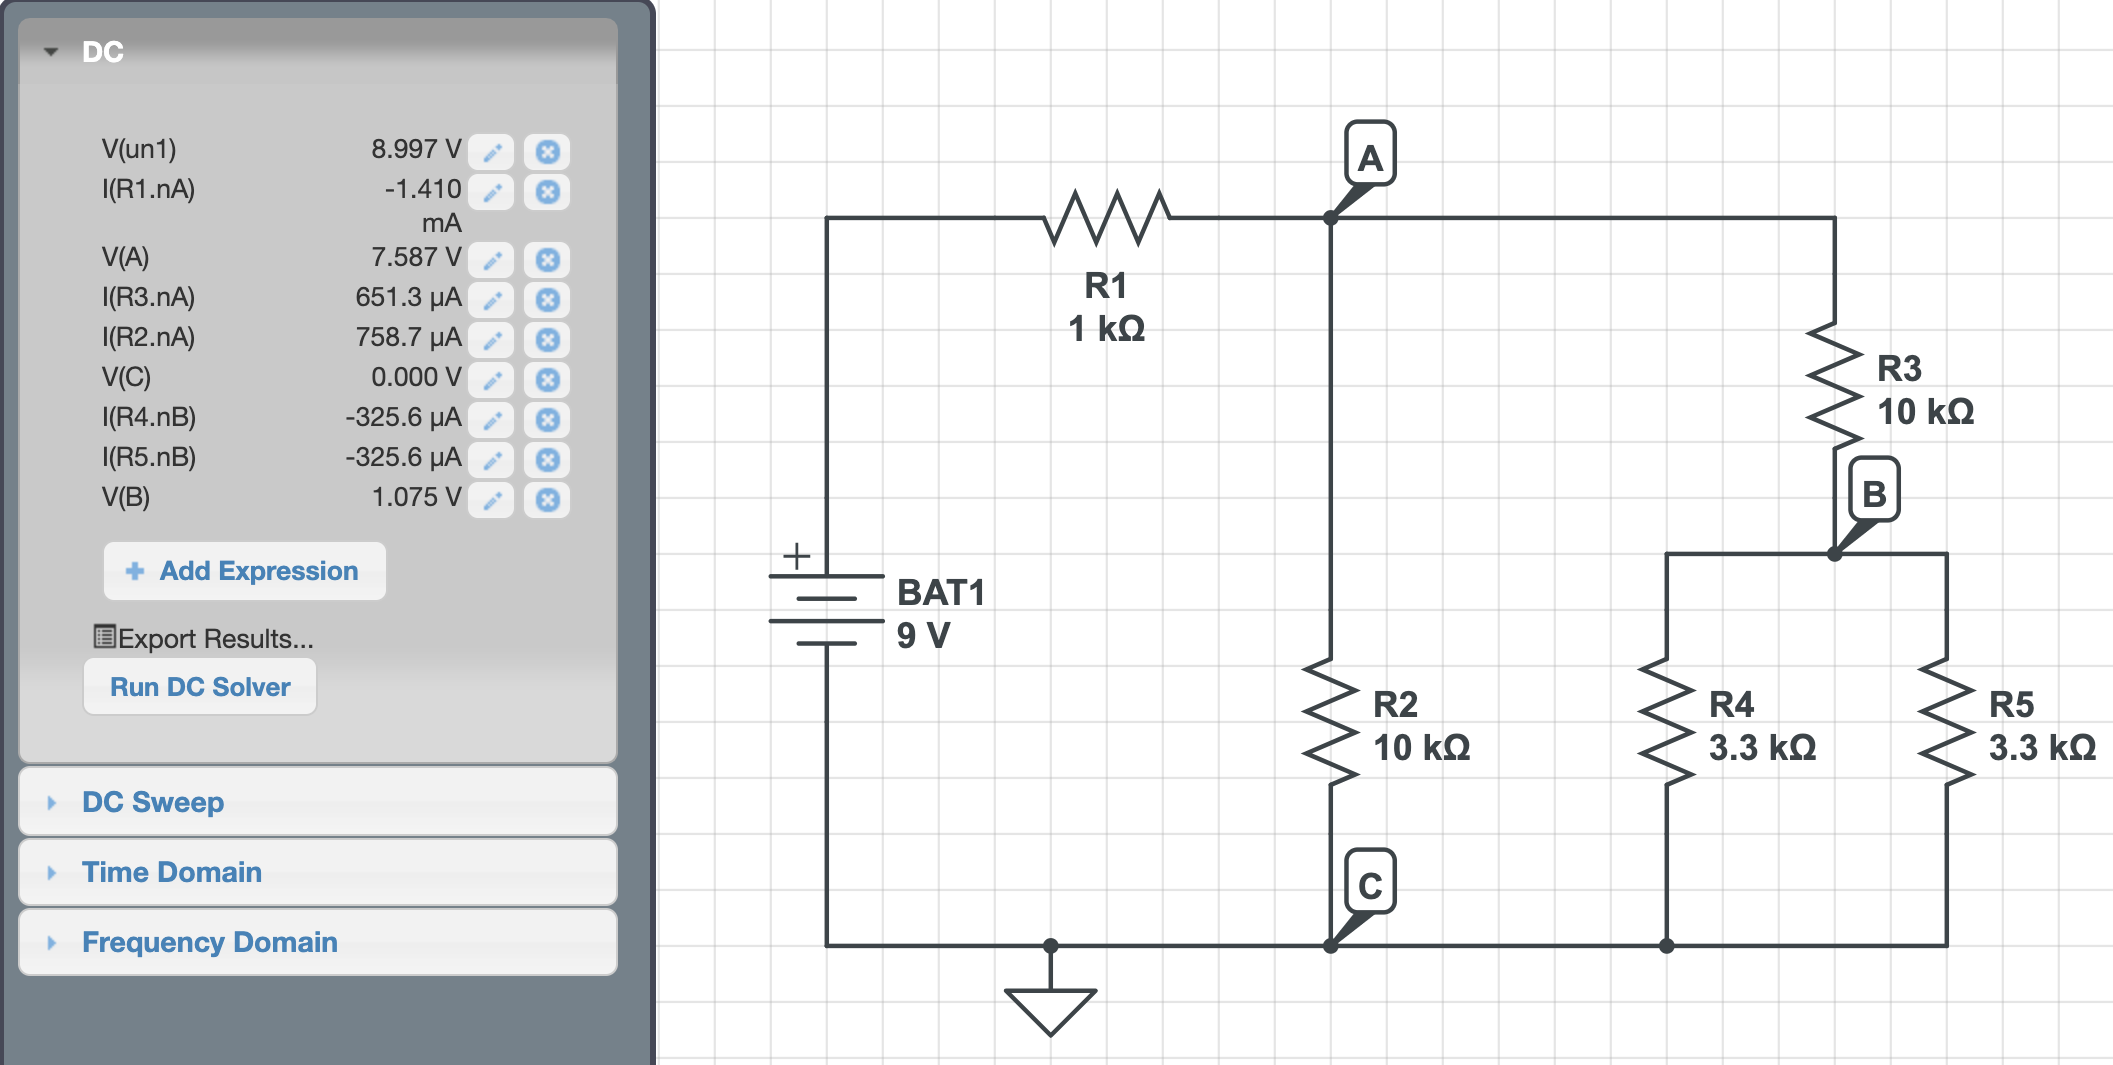
\includegraphics[scale=0.4]{vedlegg/3.png}\linebreak
                    \textit{\textcolor{gray}{Figur 4: Skjematisk oppsett av kretsen i oppgave 3. Figuren er tegnet i CircuitLab.}}
                \end{center}
            
            \subsection*{Oppg. 4:}
            Regner ut spenningen i A gitt scenario 1, 2, 3 og 4 ved bruker av formel (1):
            \begin{equation*}
                \begin{split}
                    nr. 1: R_1 &= 10\Omega \;\;\; R_2 = 10\Omega \\
                    \hline \\
                    R_{tot} &= 10\Omega + 10\Omega = 20\Omega \\
                    I &= \dfrac{9V}{20\Omega} = 0.45A \\
                    V_A &= 9V-(0.45A*10\Omega) = 4.5V \\
                    \\
                    nr. 2: R_1 &= 10\Omega \;\;\; R_2 = 1k\Omega \\
                    \hline \\
                    R_{tot} &= 10\Omega + 1k\Omega = 1010\Omega \\
                    I &= \dfrac{9V}{1010\Omega} = 8.9mA \\
                    V_A &= 9V-(8.9mA*10\Omega) = 8.911V \\
                    \\
                    nr. 2: R_1 &= 1k\Omega \;\;\; R_2 = 1\Omega \\
                    \hline \\
                    R_{tot} &= 1k\Omega + 1\Omega = 1010\Omega \\
                    I &= \dfrac{9V}{1010k\Omega} = 8.9mA \\
                    V_A &= 9V-(8.9mA*1k\Omega) = 0.1V \\
                    \\
                    nr. 2: R_1 &= 1k\Omega \;\;\; R_2 = 1k\Omega \\
                    \hline \\
                    R_{tot} &= 1k\Omega + 1k\Omega = 2\Omega \\
                    I &= \dfrac{9V}{2k\Omega} = 4.5mA \\
                    V_A &= 9V-(4.5mA*1k\Omega) = 4.5V \\
                \end{split}
            \end{equation*}

            \pagebreak
            Simulasjonen i CircuitLab:
            \begin{center}
                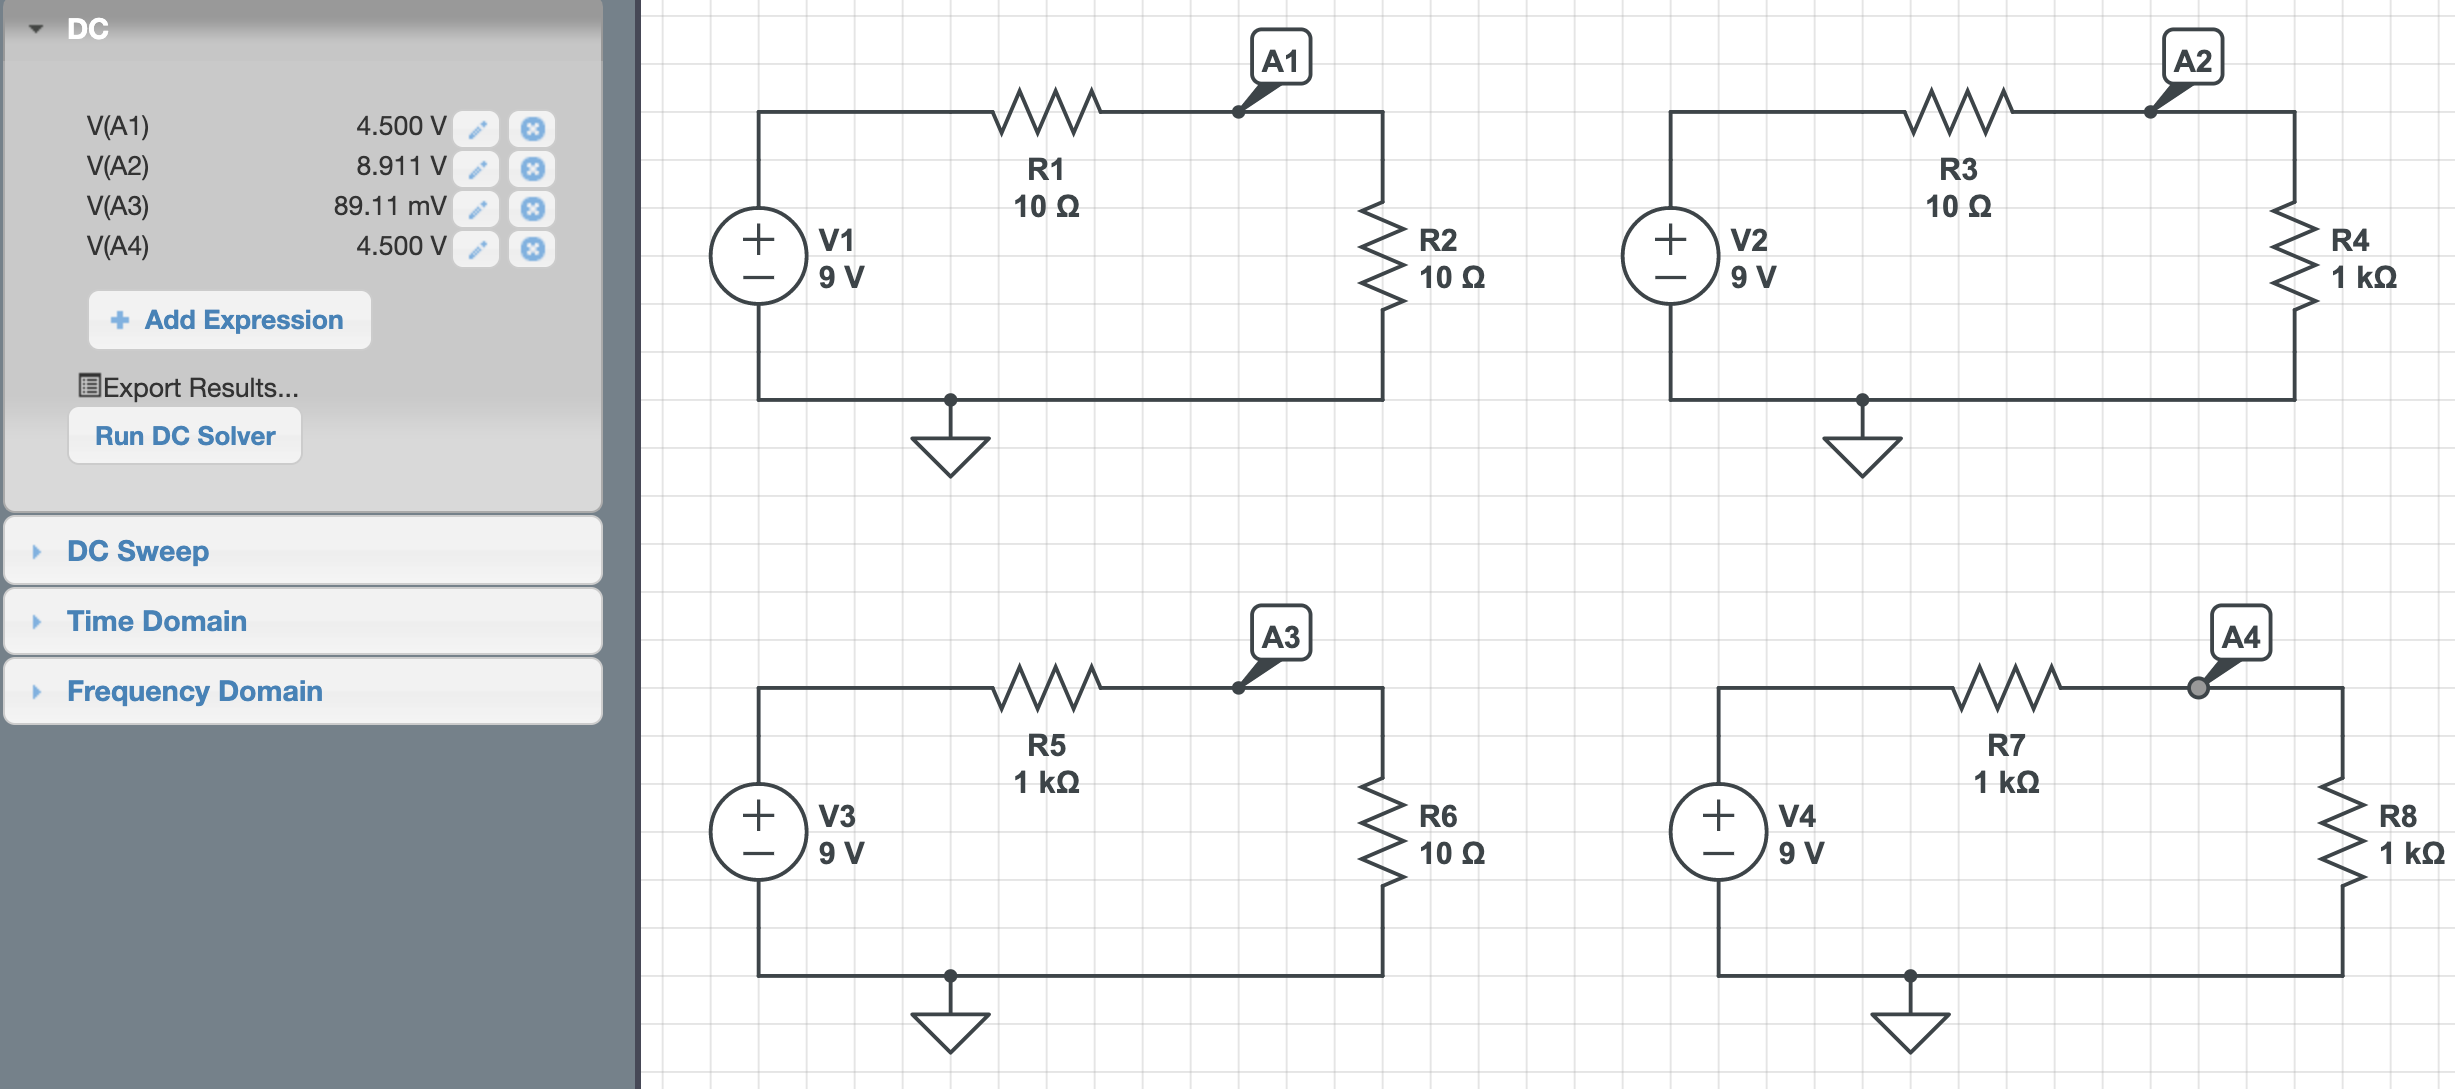
\includegraphics[scale=0.35]{vedlegg/4.png}\linebreak
                \textit{\textcolor{gray}{Figur 5: Simulering av de 4 scenarione. Figuren er tegnet i CircuitLab.}}
            \end{center}

            Kobler 2 x 1kΩ motstandere i serie til hverandre på den ene siden av brettet, og 2 x 10Ω motstandere 
            på den andre siden av brettet. Bruker deretter multimeteret for å måle spenneningen.

    \section*{4. Resultater}
        \subsection*{Oppg. 1:}
        \textbf{1a)} 
        Måleren viser 9.53v, noe som er 0.53v høyere enn forventet 9v. \linebreak

        \textbf{1b)}
        \textit{\textcolor{gray}{Tabell 1: Resultatene fra avlesningen av fargene og målingene med multimeter}}\linebreak
        \begin{center}
            \begin{tabular}{ c|c|c|c } 
             Rn & Ω - fargekoder & Ω - tolleranse & Ω - multimeter \\ 
             \hline
             R1 & 10Ω & \(\pm 1\) & 10Ω\\
             R2 & 47Ω & \(\pm 1\) & 47Ω \\
             R3 & 47Ω & \(\pm 0.1\% \) & 46.6Ω\\
             R4 & 47Ω & \(\pm 1\) & 47Ω \\
             R5 & 470Ω & \(\pm 0.1\% \) & 466Ω \\
             R6 & 470Ω & \(\pm 0.1\% \) & 466Ω \\
             R7 & 10kΩ & \(\pm 1\) & 0.99kΩ \\
             R8 & 10kΩ & \(\pm 1\) & 9.99kΩ \\
             R9 & 47kΩ & \(\pm 1\) & 46.9kΩ \\
             R10 & 100kΩ & \(\pm 0.1\% \) & 100.4kΩ
            \end{tabular}
        \end{center}
    
        \textbf{1c)} \linebreak
            › Multimeren målte 9mA \linebreak
            › Fra oppg.1 A visste vi at multimeteret viste 9.58V på batteriet og i følge farge-koden til motstanderen 
            skal toleransen ligge på \(\pm\) 0.1\%, dette førte likevell til at multimeren målte 9mA på koblingsbrettet. 
            Dette bekrefter at den analytiske, den simulerte og den målte strømmen samsvarer.
        
        \subsection*{Oppg. 2:}
            Ved å kjøre DC solver, får jeg at: \linebreak
                › V(A) = 8.994V \linebreak
                › V(B) = 6.902V » noe som indikerer en ca. 2.1V spenningsfall \linebreak
                › V(un2) = 0V » etter R2 faller spenningen til 0, altså ca. 6.9V spenningsfall \linebreak

            Siden at potensiometeret har en spenningsfall på ca.9V, kan jeg vri den til å være lik R1 og R2 ved å regne 
            ut \(1-(1/4.3)\). Dette gir ca. 0.767. \linebreak
            Når jeg vrir potensimeteret til 0.767 får jeg \(\Delta Va \approx 2.1V \) og \(\Delta Vb \approx 6.9V \). \linebreak

            På koblingsbrettet fikk jeg:
            › \(V_R1 = 7.1V \)
            › \(V_R2 = 0.2V \)

            Dette samstemmer med spenningsfall på ca. 2.1V og 6.9V over R1 og R2. 
            Optiometeren gav meg 0V hele tiden.
        
        \subsection*{Oppg. 3:}
        \textit{\textcolor{gray}{Tabell 2: Strømmene gjennom de forskjellige motstandene}}\linebreak
        \begin{center}
            \begin{tabular}{c|c|c}
                Rn & kalkulert strøm (I) & målt strøm (I) \\
                \hline
                R1 & 1.4mA & 1.6mA\\
                R2 & 0.76mA & 0.79mA\\
                R3 & 0.65mA & 0.66mA\\
                R4 & 0.33mA & 0.3mA\\
                R5 & 0.33mA & 0.3mA\\
            \end{tabular}
        \end{center}

        Som man kan lese av i tabell 2, er resultatene av simuleringen veldig lik den analystiske 
        kalkulasjonen som igjen gjenspeiles i målingene gjort med multimeteret.

        \subsection*{Oppg. 4:}
        Når jeg målte spenningen for R1 og R2 ved motstanden 1kΩ fikk jeg VA = 4.7V, og ved 
        motstand 10Ω fikk jeg VA = 4.56V.

    \section*{5. Diskusjon}
        \subsection*{Oppg. 2:}
        Optiometeren funket ikke mest sansynlig pga. av feilkobling som gjorde at strømmen aldri nådde 
        frem fra batteriet.

        \subsection*{Oppg. 3:}
        Den målte strømmen over de forskjellige motstandene varierer med batteriets ordinære spenning, 
        hvor godt koblet kretsen er og hvor stødig målepinnene ble holdt. \linebreak

        Ja: analysen, simulasjonen og målingene stemmer overens.

        \subsection*{Oppg. 4:}
        Det at målingene i oppgave 4 er litt forskjellige skyldes tolleransen i motstanderne, hvor 
        godt koblet kretsen er og hvor stødig målepinnene ble holdt. \linebreak

        Som vi så i utregningen av spenningen i punkt A, vil strømmen være størst når gjennom 
        kretsen når R1 = R2. For å få maksimal effektoverføring, må R2 derfor være lik R1.
    \section*{6. Konklusjon}
        \begin{verbatim}
        Denne rapporten viser mitt arbeid med Lab 1, hvor jeg 
        etter beste evne har prøvd å finne og bruke matematiske 
        teorier for så å simulere dem også til slutt lage reelle 
        kretser. Jeg oppdaget underveis hvor viktig det er å bli 
        godt kjent med verktøyene man skal bruke, spesielt når man 
        måler små verdier og størrelser.
    \end{verbatim}
\end{document}